
\section{Задание 9}

Рассмотреть два вида процессов:
\begin{itemize}
	\item Винеровский процесс $W(t), t \in [0,1], W(0) = 0$.
	\item Процесс Орнштейна--Уленбека $X(t), t \in [0,1], X(0) = X_0$, то есть 
    стационарный марковский гауссовский процесс. Начальные значения $X_0$ 
    генерируются случайным образом так, чтобы полученный процесс был 
    стационарным.
\end{itemize}

Для данных гауссовских процессов
\begin{enumerate}
	\item Найти ковариационную функцию и переходные вероятности.
	\item Моделировать независимые траектории процесса с данными переходными 
    вероятностями методом добавления разбиения отрезка.
	\item Построить график траектории, не соединяя точки ломаной, с целью 
    получения визуально непрерывной линии.
\end{enumerate}

\subsection{Винеровский процесс}

    По определннию (\cite{SAIM}) ковариационная функция Винеровского процесса 
    $W_t$ имеет вид $\cov(t,s) = \min (t,s)$. Плотность многомерного 
    нормального распределения $\mathcal{N}(m,R)$
    \begin{equation*}
        p(x) = \frac{1}{(2\pi)^
        {\frac{n}{2}}\sqrt{|R|}}e^ {-\frac{1}{2}(x-m)^T R^{-1}(x-m)},
    \end{equation*}
    где $R$ --- ковариационная матрица. Для моделирования Винеровского процесса 
    достаточно знать, что $W_0 = 0, W_1 \sim \mathcal{N}(0,1)$ и для $t_0, t_1, 
    \alpha \in (0,1)$ условное распределение в момент $t = (1-\alpha)t_0 + 
    \alpha t_1$ имеет плотность
    \begin{equation*}
        p_{W_t \mid W_{t_0},W_{t_1}} (x \mid x_0,x_1) = 
        \frac{p_{W_{t_0},W_t,W_{t_1}}(x_0,x,x_1)} {p_{W_{t_0},W_{t_1}}(x_0,x_1)},
	\end{equation*}
    где
    \begin{gather*}
        p_{W_{t_0},W_t,W_{t_1}} = \frac{1}{(2\pi)^{\frac{3}{2}}\sqrt{|R_3|}} 
        e^{-\frac{1}{2}x^T R_3^{-1} x},\\
        p_{W_{t_0},W_{t_1}} = 
        \frac{1}{(2\pi)\sqrt{|R_2|}} e^{-\frac{1}{2}x^T R_2^{-1} x},\\
        R_3 = \begin{pmatrix}
                t_0 & t_0 & t_0 \\
                t_0 & t & t \\
                t_0 & t & t_1
                \end{pmatrix} ,
        R_2 = \begin{pmatrix}
            t_0 & t_0 \\
            t_0 & t_1
            \end{pmatrix}.        
    \end{gather*}

    Отсюда
    \begin{equation*}
        p_{W_t \mid W_{t_0},W_{t_1}} (x \mid x_0,x_1) = 
        \frac{1}{\sqrt{2\pi\alpha(1-\alpha)(t_1-t_0)}} 
        e^{\displaystyle{-}
        \dfrac{(x-((1-\alpha)x_0+\alpha x_1))^2}{2\alpha(1-\alpha)(t_1-t_0)}},
    \end{equation*}
    т.е. $W_t \sim \mathcal{N}(x,\alpha(1-\alpha)(t_1 - t_0))$. В случае 
    $\alpha = \frac{1}{2}$ $W_t \sim \mathcal{N}(x,\frac{t_1-t_0}{4})$

    Таким образом, для моделирования Винеровского процесса достаточно получить 
    некоторые значения $W_0 = 0$, $W_1 \sim \mathcal{N}(0,1)$, и затем 
    последовательно методом бисекции разыгрывать величины $W_t \sim 
    \mathcal{N}(x,\frac{t_1-t_0}{4})$.

\subsection{Процесс Орнштейна-Уленбека}

    Из стационарности процесса Орнштейна-Уленбека $X_t$ следует, что 
    $\Exp X_t = a$, $\Disp X_t = \sigma^2$ и
    \begin{equation*}
        \cov (X_t,X_s) = \sigma^2 \rho(x,y) = \sigma^2 \rho(x) \rho(y) = 
        \sigma^2 e^{-\theta(x+y)}
    \end{equation*}

    Условное распределение имеет вид $(X_t \mid X_s = x) \sim 
    \mathcal{N}(x e^{\theta |t-s|},\:\sigma^2(1-e^{-2\theta |t-s|}))$.

    Процесс Орнштейна-Уленбека моделируется так же как и Винеровский, лишь с 
    учетом того, что $X_0 \sim \mathcal{N}(a,\sigma^2)$, 
    $X_1 \sim \mathcal{N}(x_0 e^{-\theta T}, \sigma^2 (1-e^{-2\theta T}))$, и
    \begin{equation*}
        X_{\frac{t_0 + t_1}{2}} \sim \mathcal{N}\left( 
            (x_0+x_1)\frac{e^\frac{-\theta(t_1-t_0)}{2}}{1 + e^{-\theta(t_1-t_0)}},\:
            \sigma^2 \frac{1 - e^{-\theta(t_1-t_0)}}{1 + e^{-\theta(t_1-t_0)}} 
            \right)
    \end{equation*}

    Результат моделирования процессов см. рис. \ref{processes}

    \begin{figure}[tbp]
        \centering
        \begin{subfigure}[b]{0.48\textwidth}
            \centering
            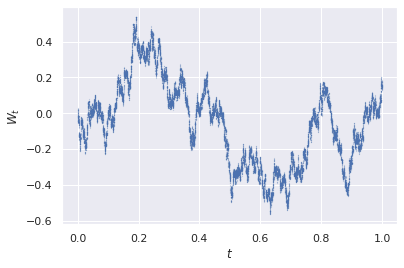
\includegraphics[width=\textwidth]{resources/task9_Wiener.png}
            \caption{Винеровский процесс}
        \end{subfigure}
        \hfill
        \begin{subfigure}[b]{0.48\textwidth}
            \centering
            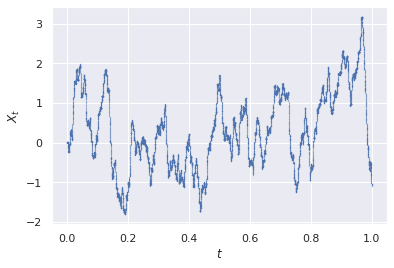
\includegraphics[width=\textwidth]{resources/task9_OrnUhl.png}
            \caption{Процесс Орнштейна-Уленбека}
        \end{subfigure}
        \caption{}
        \label{processes}
    \end{figure}